\documentclass[margin=10pt]{standalone}
\usepackage{pgfplots}
\pgfplotsset{compat=1.18}
\usetikzlibrary{arrows.meta}

\begin{document}

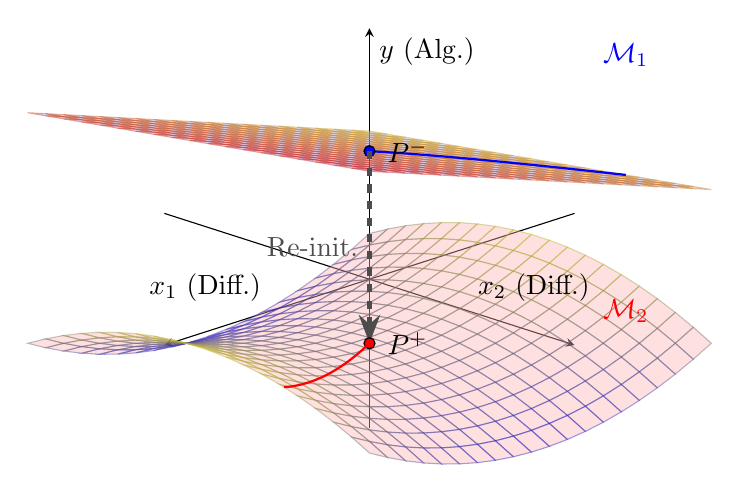
\begin{tikzpicture}
\begin{axis}[
    view={120}{30}, % Adjust the perspective
    width=12cm,
    height=10cm,
    xlabel={$x_1$ (Diff.)},
    ylabel={$x_2$ (Diff.)},
    zlabel={$y$ (Alg.)},
    axis lines=center,
    grid=major,
    ticks=none,
    enlargelimits=0.1,
    view={135}{25}
]

% --- Manifold M1 (Pre-switch) ---
\addplot3[
    surf, 
    opacity=0.4, 
    fill=blue!30, 
    draw=blue!50,
    domain=-2:2, 
    y domain=-2:2,
    samples=20
] {0.5*x + 0.2*y + 2};
\node[blue] at (axis cs: -1.5, 1.5, 3.5) {$\mathcal{M}_1$};

% --- Manifold M2 (Post-switch) ---
\addplot3[
    surf, 
    opacity=0.4, 
    fill=red!30, 
    draw=red!50,
    domain=-2:2, 
    y domain=-2:2,
    samples=20
] {0.2*x^2 - 0.2*y^2 - 1};
\node[red] at (axis cs: -1.5, 1.5, -0.5) {$\mathcal{M}_2$};

% --- Points and Trajectories ---

% 1. Pre-switch Point P- and trajectory
\addplot3[blue, thick, samples y=0, domain=-2:0] ({x}, {x^2/4}, {0.5*x + 0.2*(x^2/4) + 2});
\draw[fill=blue] (axis cs: 0, 0, 2) circle (2pt) node[right, xshift=3pt] {$P^-$};

% 2. The JUMP (Re-initialization)
% This line is strictly vertical, meaning x variables are constant
\draw[ultra thick, dashed, -{Stealth}, black!70] (axis cs: 0, 0, 2) -- (axis cs: 0, 0, -1)
    node[midway, left] {Re-init.};

% 3. Post-switch Point P+ and trajectory
\draw[fill=red] (axis cs: 0, 0, -1) circle (2pt) node[right, xshift=3pt] {$P^+$};
\addplot3[red, thick, samples y=0, domain=0:2] ({x}, {x/2}, {0.2*x^2 - 0.2*(x/2)^2 - 1});

\end{axis}
\end{tikzpicture}

\end{document}